%!TEX root = paper.tex
%%%%%%%%%%%%%%%%%%%%%%%%%%%%%%%%%%%%%%%%%%%%%%%%%%%%%%%%%%%%%%%%%%%%%%%%%%%%%%%%
\section{Overwatch Lag Simulation}
\label{sec:simulation}

\begin{figure}
	\centering
	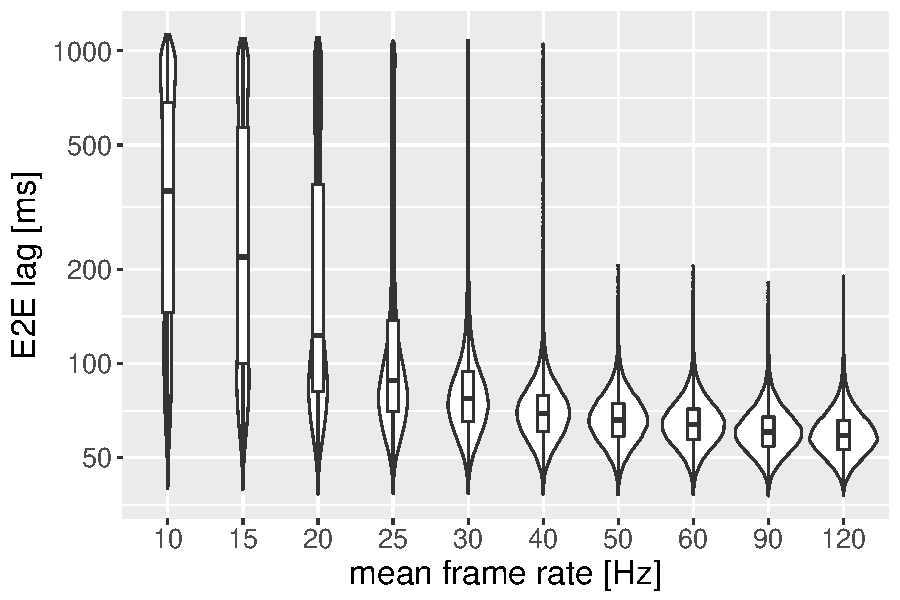
\includegraphics[width=1.0\columnwidth]{images/lagsim.pdf}
	\caption{\acrshort{E2E} lag results of a frame rate study using the \textsc{Overwatch} simulation. The denoted frame rates are the mean of the normal distribution.}
\label{fig:lagsim}
\end{figure}

% TODO: - Interpretation of Figure 5: what happens between 40 and 50 Hz (when the maximal E2E lag suddenly decreases from >1 s to >200 ms)? Why such an abrupt change?
% TODO: Why is there such a spread in the second phase? --- Answer we honestly do not know, but might be attributed to internal game behavior

Now that all client-observable parameters have been examined, a simulation study is performed on the effects of the game's frame rate. This the only direct game parameter that the player can influence through the game's setting or through more capable hardware that influences the lag. But, since it is often tricky to maintain a stable frame rate in such resource constrained environments, the frame rate in this simulation is modeled as a normal distribution instead of a fixed value. This should account for the variations in the frame times (the time between two consecutive frames). Investigated here were frame rates between \SI{10}{\hertz} and \SI{120}{\hertz}. The minimum value might occur in high stress situations when resource are severely constrained, and the maximum value representing what can be achieved with modern PC hardware and monitors. All other simulation parameters are derived from the models in the previous section or left as-is in the base simulation. 

The results are depicted in Fig.~\ref{fig:lagsim}. Starting at about \SI{50}{\hertz} the \gls{E2E} lag reduction sees diminishing returns especially towards its outliers, which can exceed a lag of over a second below \SI{50}{\hertz}. This correlates quite well with the generally accepted notion that (especially) online first person shooters require at least \SI{60}{\hertz} for an enjoyable experience. In praxis, only \SI{30}{\hertz}, \SI{60}{\hertz} or higher frame rates will be targeted, due to otherwise occurring interactions with the monitor's refresh rate, which results in either screen tearing or an unstable \gls{IAT} of the rendered frames.
